




\begin{frame}
\frametitle{Graphics Jpeg Dataset Scatter Psnr[db] vs Bpp}

\begin{columns}
\column{0.5\textwidth}
\begin{figure}
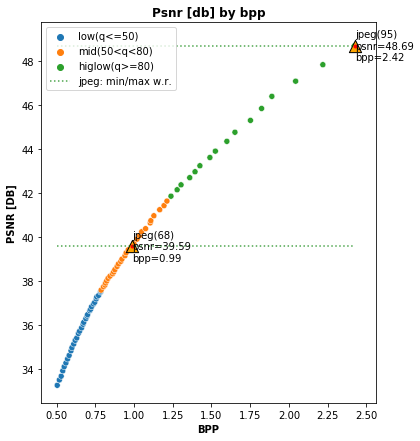
\includegraphics[scale=0.35]{slides/experiments/jpeg_dataset/jpeg_bpp_vs_psnr_scatter_gby_param_class.png}
\caption{Scatter Plot Psnr [db] vs Bpp for Jpeg Dataset.}
\end{figure}
\column{0.5\textwidth}
Here, it is reported a Scatter plot, where on the x-axis was located Bpp, while on y-axis was set Peak-Signal-to-Noise-Ration, shortly Psnr, expressed in decibel, where the highere
the Psnr score the better the algorithm was ebla to keep signa data over noise introduced by the procedure itself; whereas speaking about Bpp metric, we know that the lower the score
the better the compressing procedure was able to keep meaningful signal information while reducing the number of pixels needed to represent the overall compressed image.
\end{columns}

\end{frame}